
\chapter{Flugleistungen}

\deftripstyle{Flughandbuch}[.5pt][.5pt]{\pagemark}{}{\headmark}{Flug- und Betriebshandbuch B13}{}{05.2013}
\pagestyle{Flughandbuch}
\renewcommand*\chapterpagestyle{Flughandbuch}


\section{Einführung}
Abschnitt 5 enthält anerkannte Daten für die Berichtigung der Fahrtmesseranzeige und die Überziehgeschwindigkeiten für unterschiedliche Klappenstellungen sowie weitere, nicht anerkannte Angaben.
\newpage


\subsection{Nachgewiesene Seitenwindkomponenten}
Noch nicht nachgewiesen.
%\begin{tabular}{l l}
%Windenstart: & ?$\frac{km}{h}$\\
%Flugzeugschlepp: & ?$\frac{km}{h}$\\
%Landung: & ?$\frac{km}{h}$\\
%
%\end{tabular}
\section{Geschwindigkeitspolare}
Die Leistungsvermessung der B13 fand im August 1992 in Aalen-Elchingen statt. Die Flugmasse (Rüstmasse+$180kg$) lag bei $765 kg$, was einer Flächenbelastung von $\frac{G}{S}=396 \frac{N}{m^2}$ entspricht. \\
\newline
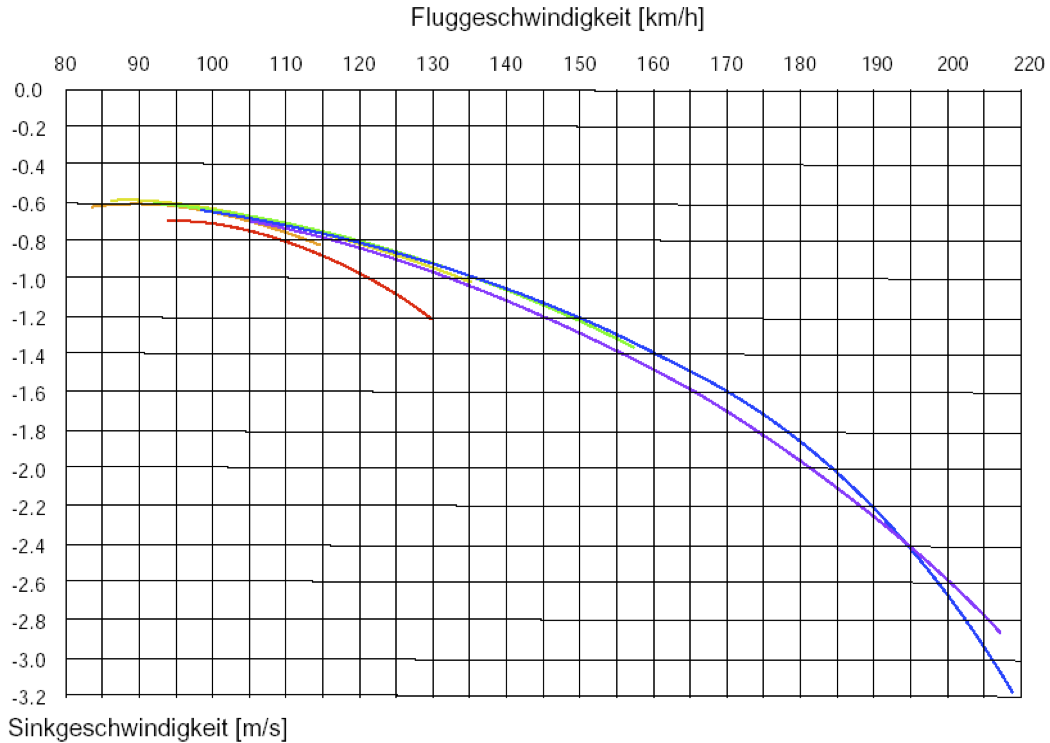
\includegraphics[width=\textwidth]{polare.png}
\newline
\begin{center}
\begin{tabular}{|c|c|c|}
\hline
Wölbklappenstellung & WK-Innen & WK-Außen\\
\hline
\begin{color}{red} L \end{color} & \begin{color}{red} $15,8^{\circ}$ \end{color} & \begin{color}{red} $11,5^{\circ}$ \end{color}\\
\hline
\begin{color}{orange} $+2$ \end{color} & \begin{color}{orange} $10,4^{\circ}$ \end{color} & \begin{color}{orange} $7,5^{\circ}$ \end{color}\\
\hline
\begin{color}{yellow} $+1$ \end{color} & \begin{color}{yellow} $4,5^{\circ}$ \end{color} & \begin{color}{yellow} $3,2^{\circ}$ \end{color}\\
\hline
\begin{color}{cyan} $0$ \end{color} & \begin{color}{cyan} $0^{\circ}$ \end{color} & \begin{color}{cyan} $0^{\circ}$ \end{color}\\
\hline
\begin{color}{blue} $-1$ \end{color} & \begin{color}{blue} $-4,3^{\circ}$ \end{color} & \begin{color}{blue} $-3,2^{\circ}$ \end{color}\\
\hline
\begin{color}{violet} $-2$ \end{color} & \begin{color}{violet} $-9,7^{\circ}$ \end{color} & \begin{color}{violet} $-7,3^{\circ}$ \end{color}\\
\hline

\end{tabular}
\end{center}
\section{Gleitzahlpolare}
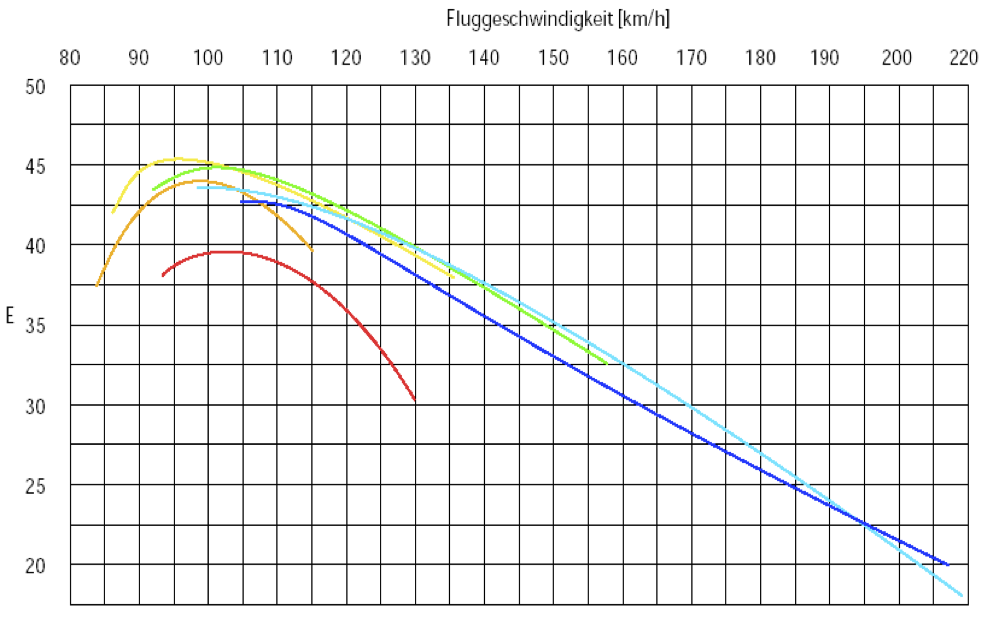
\includegraphics[width=\textwidth]{gzpolare.png}
\newline
\begin{center}
\begin{tabular}{|c|c|c|}
\hline
Wölbklappenstellung & WK-Innen & WK-Außen\\
\hline
\begin{color}{red} L \end{color} & \begin{color}{red} $15,8^{\circ}$ \end{color} & \begin{color}{red} $11,5^{\circ}$ \end{color}\\
\hline
\begin{color}{orange} $+2$ \end{color} & \begin{color}{orange} $10,4^{\circ}$ \end{color} & \begin{color}{orange} $7,5^{\circ}$ \end{color}\\
\hline
\begin{color}{yellow} $+1$ \end{color} & \begin{color}{yellow} $4,5^{\circ}$ \end{color} & \begin{color}{yellow} $3,2^{\circ}$ \end{color}\\
\hline
\begin{color}{cyan} $0$ \end{color} & \begin{color}{cyan} $0^{\circ}$ \end{color} & \begin{color}{cyan} $0^{\circ}$ \end{color}\\
\hline
\begin{color}{blue} $-1$ \end{color} & \begin{color}{blue} $-4,3^{\circ}$ \end{color} & \begin{color}{blue} $-3,2^{\circ}$ \end{color}\\
\hline
\begin{color}{green} $-2$ \end{color} & \begin{color}{green} $-9,7^{\circ}$ \end{color} & \begin{color}{green} $-7,3^{\circ}$ \end{color}\\
\hline

\end{tabular}
\end{center}
\newpage
\section{Leistungsoptimale Wölbklappenbedienung}
Auf Grundlage der Polaren ergeben sich für die verschiedenen Manöver die optimalen Wölbklappenstellungen:\\
\newline
\begin{tabular}{|m{3,5cm}|m{2cm}|m{4cm}|}
\hline
Verwendung & WK-Stellung & Geschwindigkeit [$\frac{km}{h}$]\\
\hline
langsames Kreisen in Ruhiger Thermik & $+2$ & $85$ bis $100$\\
\hline
schnelleres Kreisen in der Thermik, bestes Gleiten, geringstes Sinken & $+1$ & $90$ bis $105$\\
\hline
Gleitflug zwischen Aufwinden & $0$ & $100$ bis $135$\\
\hline
Gleitflug mit erhöhter Geschwindigkeit & $-1$ & $130$ bis $195$\\
\hline
schneller Gleitflug & $-2$ & $190$ bis $220$\\
\hline
\end{tabular}\\
\newline
\newline
Bei Erhöhung der Flächenbelastung und der Schräglage im Kreisflug erhöhen sich auch die Geschwindigkeiten.